\subsection{ Datasets}
Several publicly available datasets from Roboflow are used for the training process:

\begin{itemize}
    \item Paint damage dataset (67 images)
    \item Crack detection dataset (1551 images)
    \item House damage dataset (3570 images)
    \item Asbestos dataset (1331 images)
\end{itemize}

These datasets provide additional labeled examples of inspection-related defects and help improve model robustness during training.

\section{Inspection Category Definitions}

The following categories are used for annotation and evaluation during the experiments.

\begin{table}[H]
\centering
\begin{tabular}{|p{3cm}|p{8cm}|}
\hline
\textbf{Category} & \textbf{Description} \\
\hline
Damage & Visible structural damage such as cracks, holes, or broken surfaces. \\
\hline
Wear & Gradual deterioration of surfaces such as paint wear or discoloration. \\
\hline
Alteration & Unauthorized modifications or added structures within the property. \\
\hline
No Damage & No visible inspection-relevant issues present. \\
\hline
\end{tabular}
\caption{Inspection category definitions used during annotation and evaluation.}
\label{tab:inspection_categories}
\end{table}

\section{Annotation Procedure}

DGW images are not annotated at the start of the project. A subset of the dataset will be manually annotated during the project using bounding boxes corresponding to the predefined inspection categories.

The annotation process follows these steps:

\begin{enumerate}
    \item Selection of images from the DGW archive.
    \item Manual annotation of inspection-relevant objects using bounding boxes.
    \item Validation of annotations to ensure consistency across categories.
\end{enumerate}

Annotation is performed using assisted labeling tools in Roboflow, which allow automated suggestions followed by manual correction.

\section{LLaVA Prompt Templates}

The vision-language model LLaVA is evaluated using fixed prompt templates to ensure reproducibility.

Example prompts include:

\begin{itemize}
    \item ``Identify visible damage in this image.''
    \item ``Is there evidence of wear or alterations in this room?''
    \item ``Describe any inspection-relevant issues visible in the image.''
\end{itemize}

Model responses are mapped to the predefined inspection categories to allow comparison with the outputs of the YOLOv8 detector.

\begin{figure}[H]
    \centering

    % Row 1
    \begin{minipage}{0.32\textwidth}
        \centering
        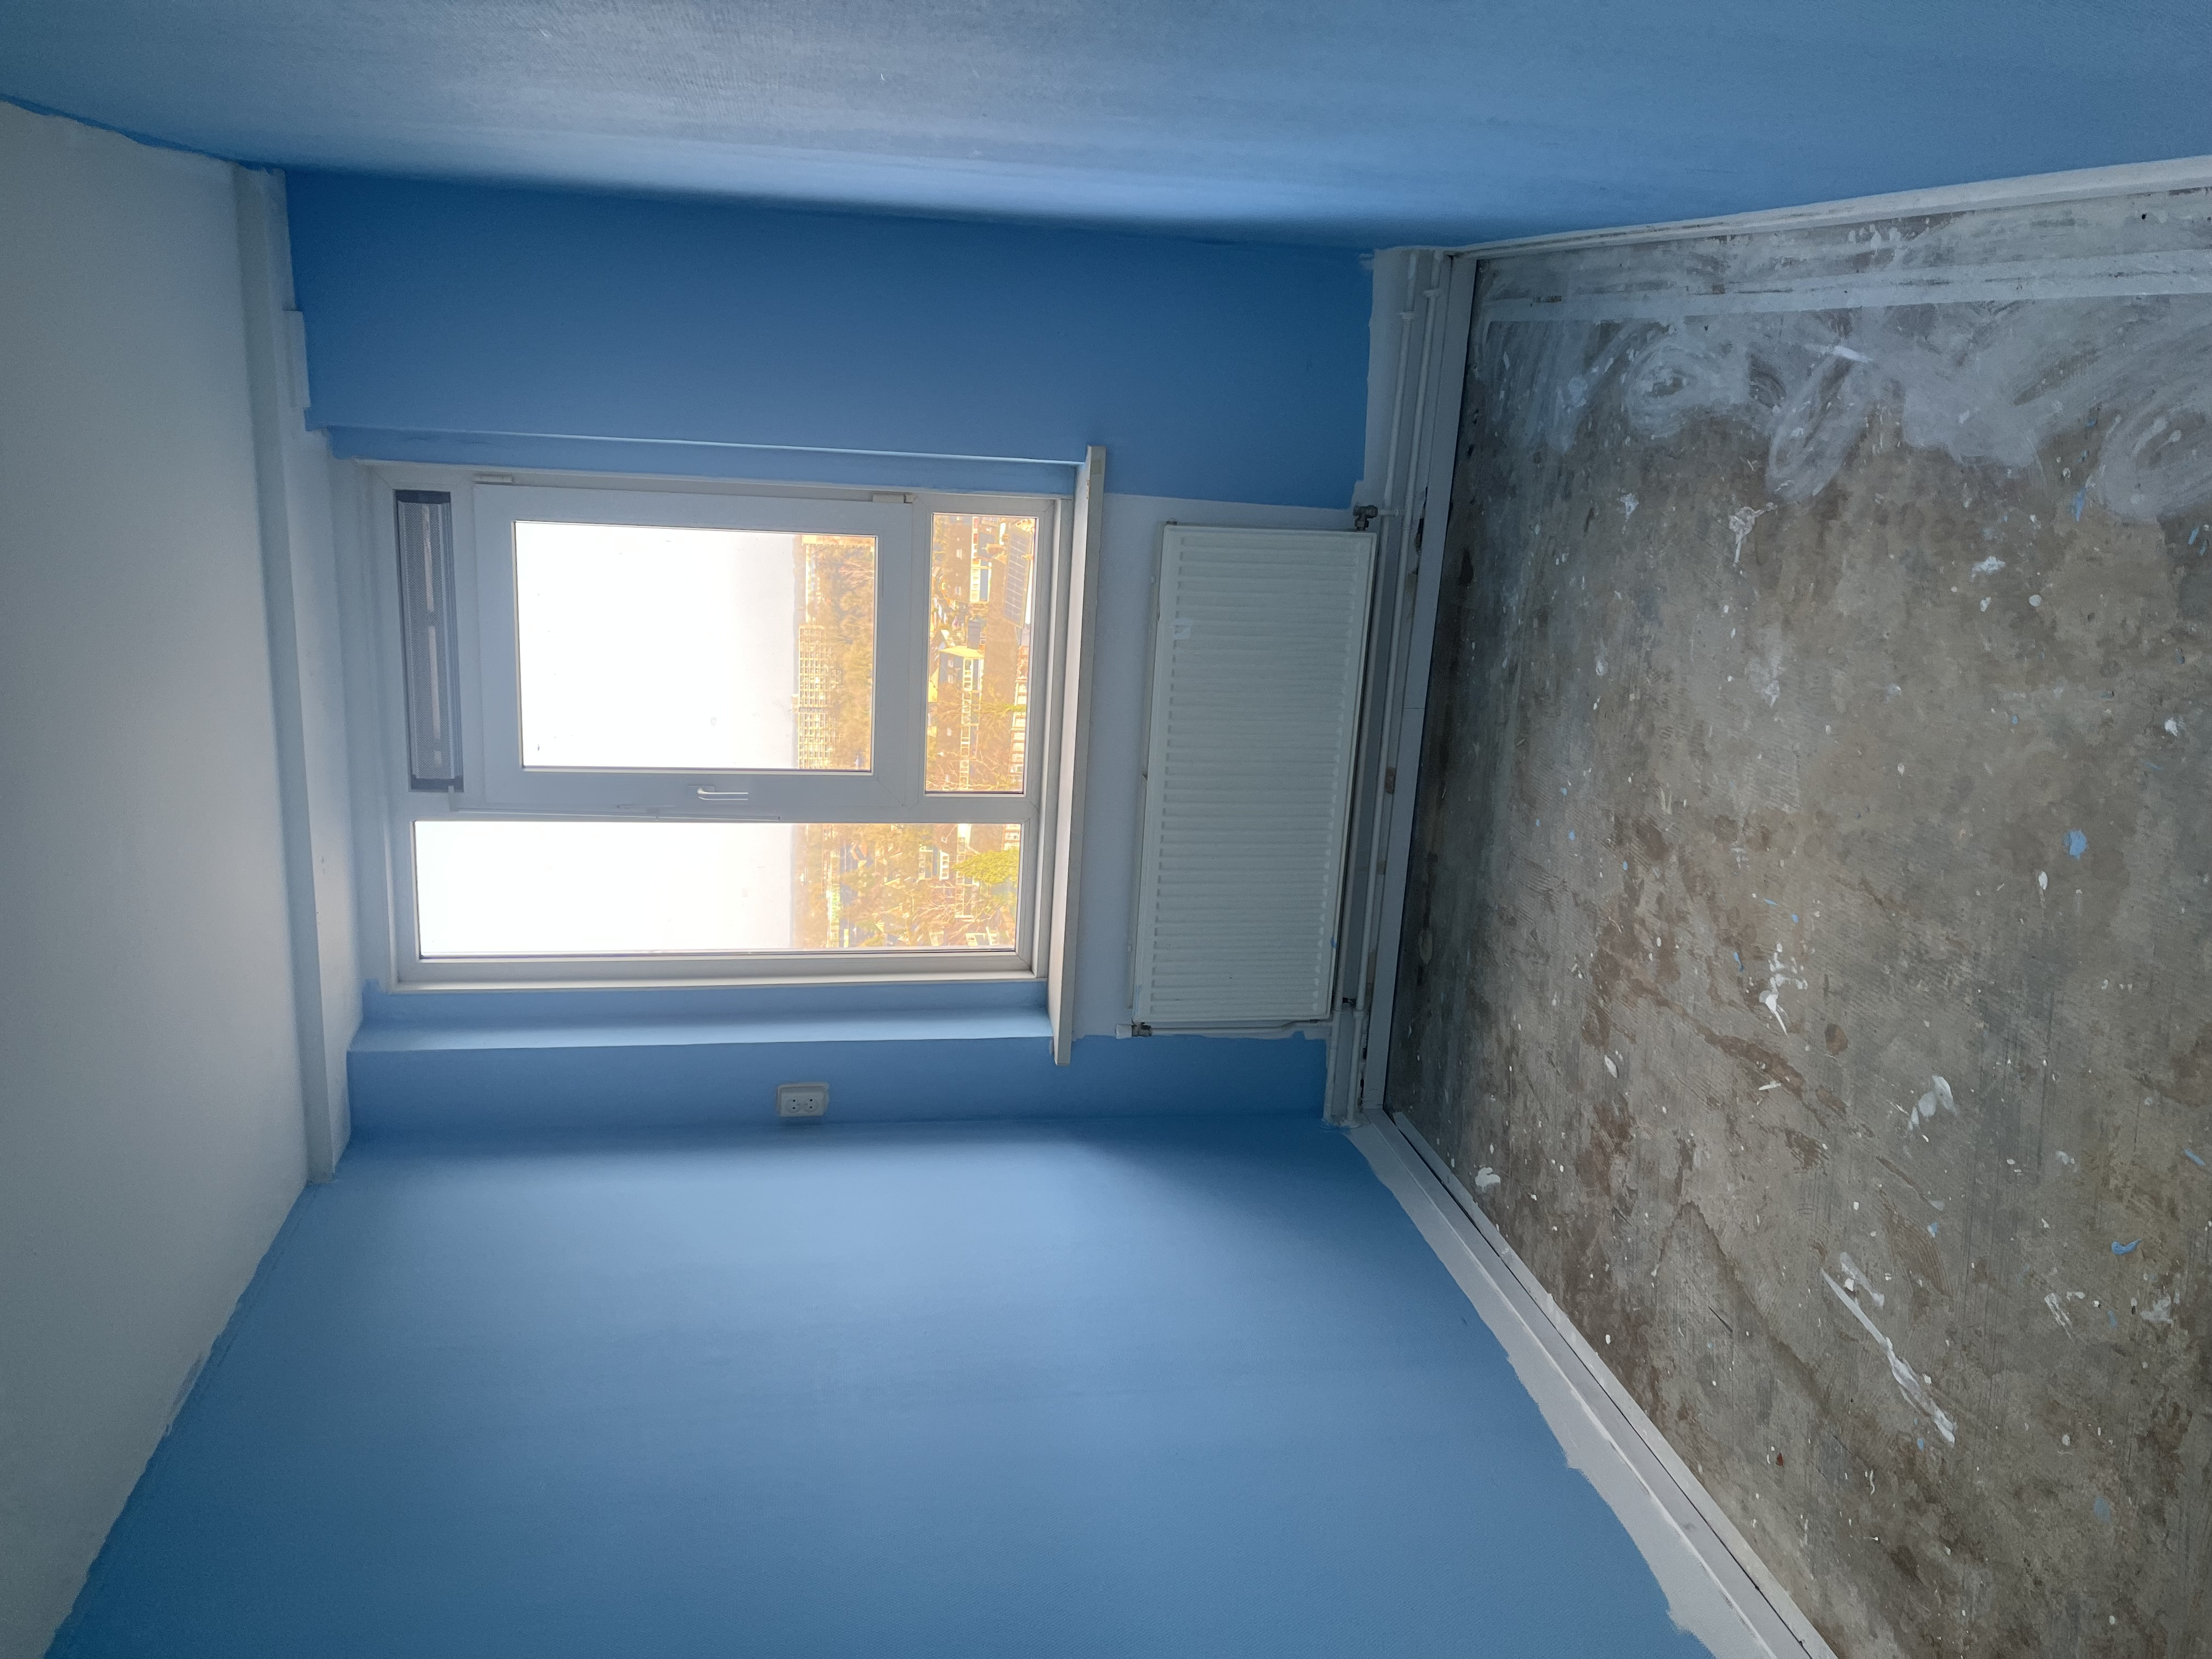
\includegraphics[angle=270,width=\linewidth]{sections/1-thesis-design/geen_schade.jpg}

        \small (a) No visible damage
    \end{minipage}\hfill
    \begin{minipage}{0.32\textwidth}
        \centering
        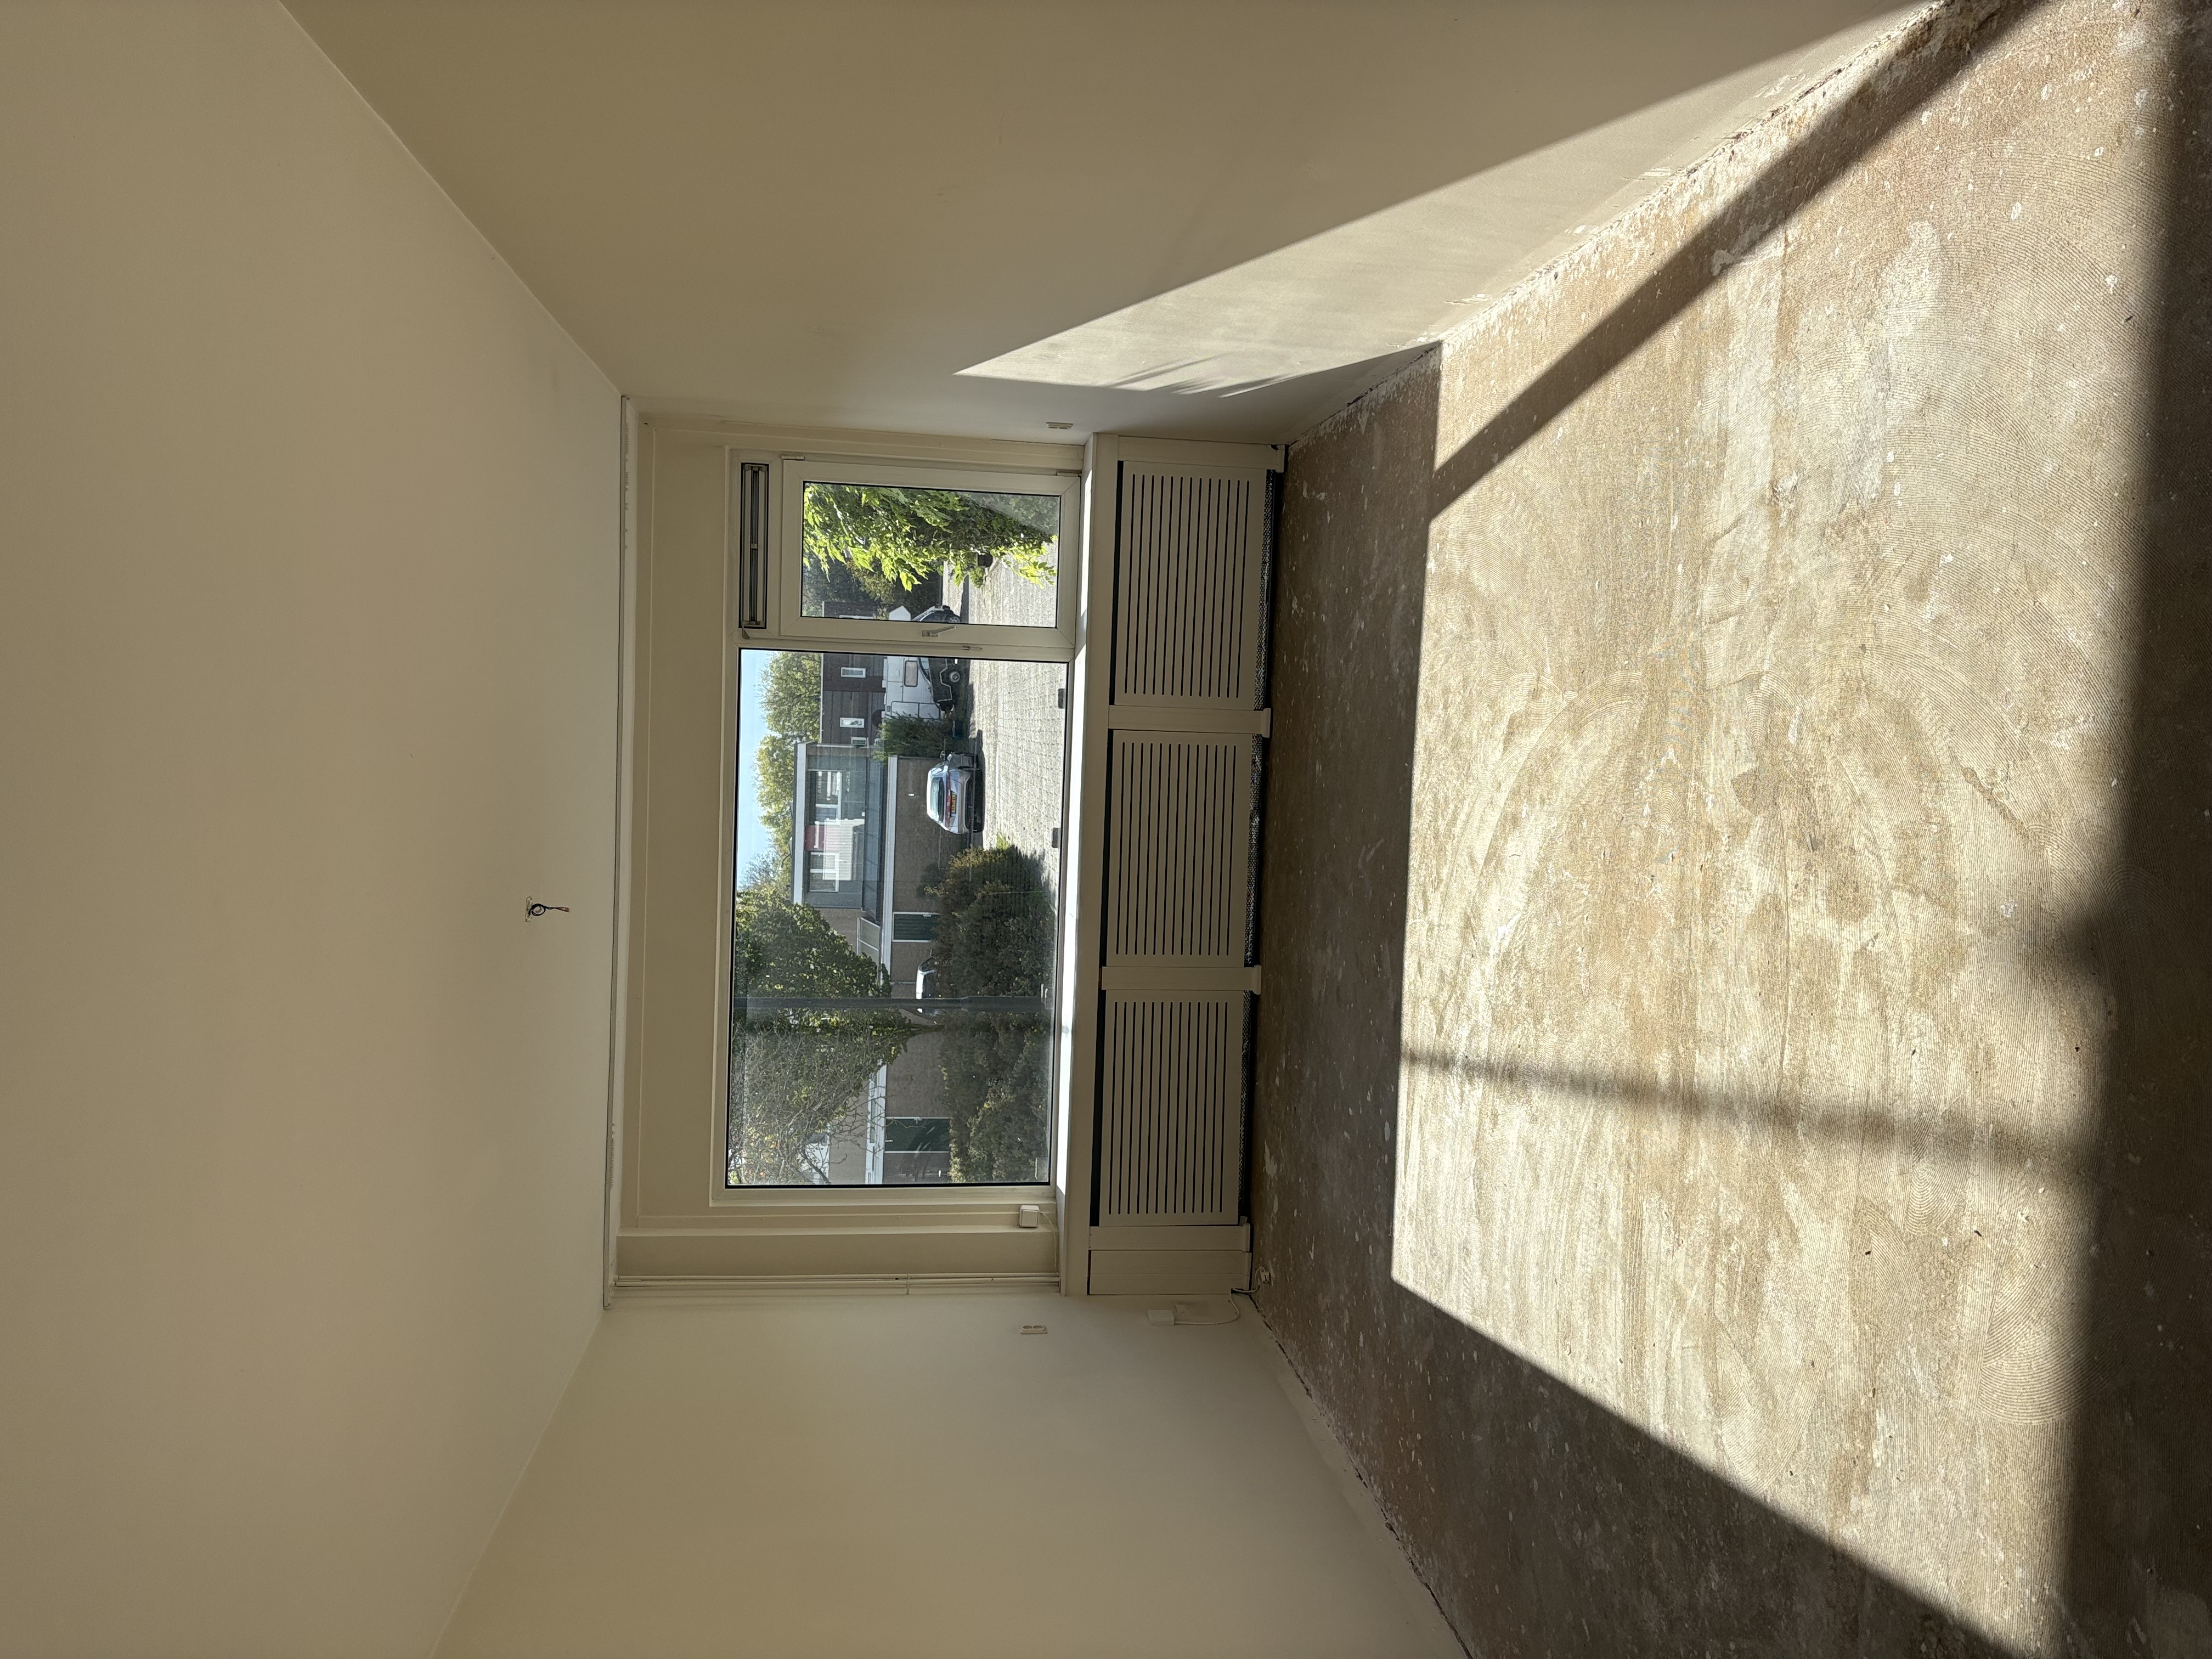
\includegraphics[angle=270,width=\linewidth]{sections/1-thesis-design/geenschade2.jpg}

        \small (b) Clean room
    \end{minipage}\hfill
    \begin{minipage}{0.32\textwidth}
        \centering
        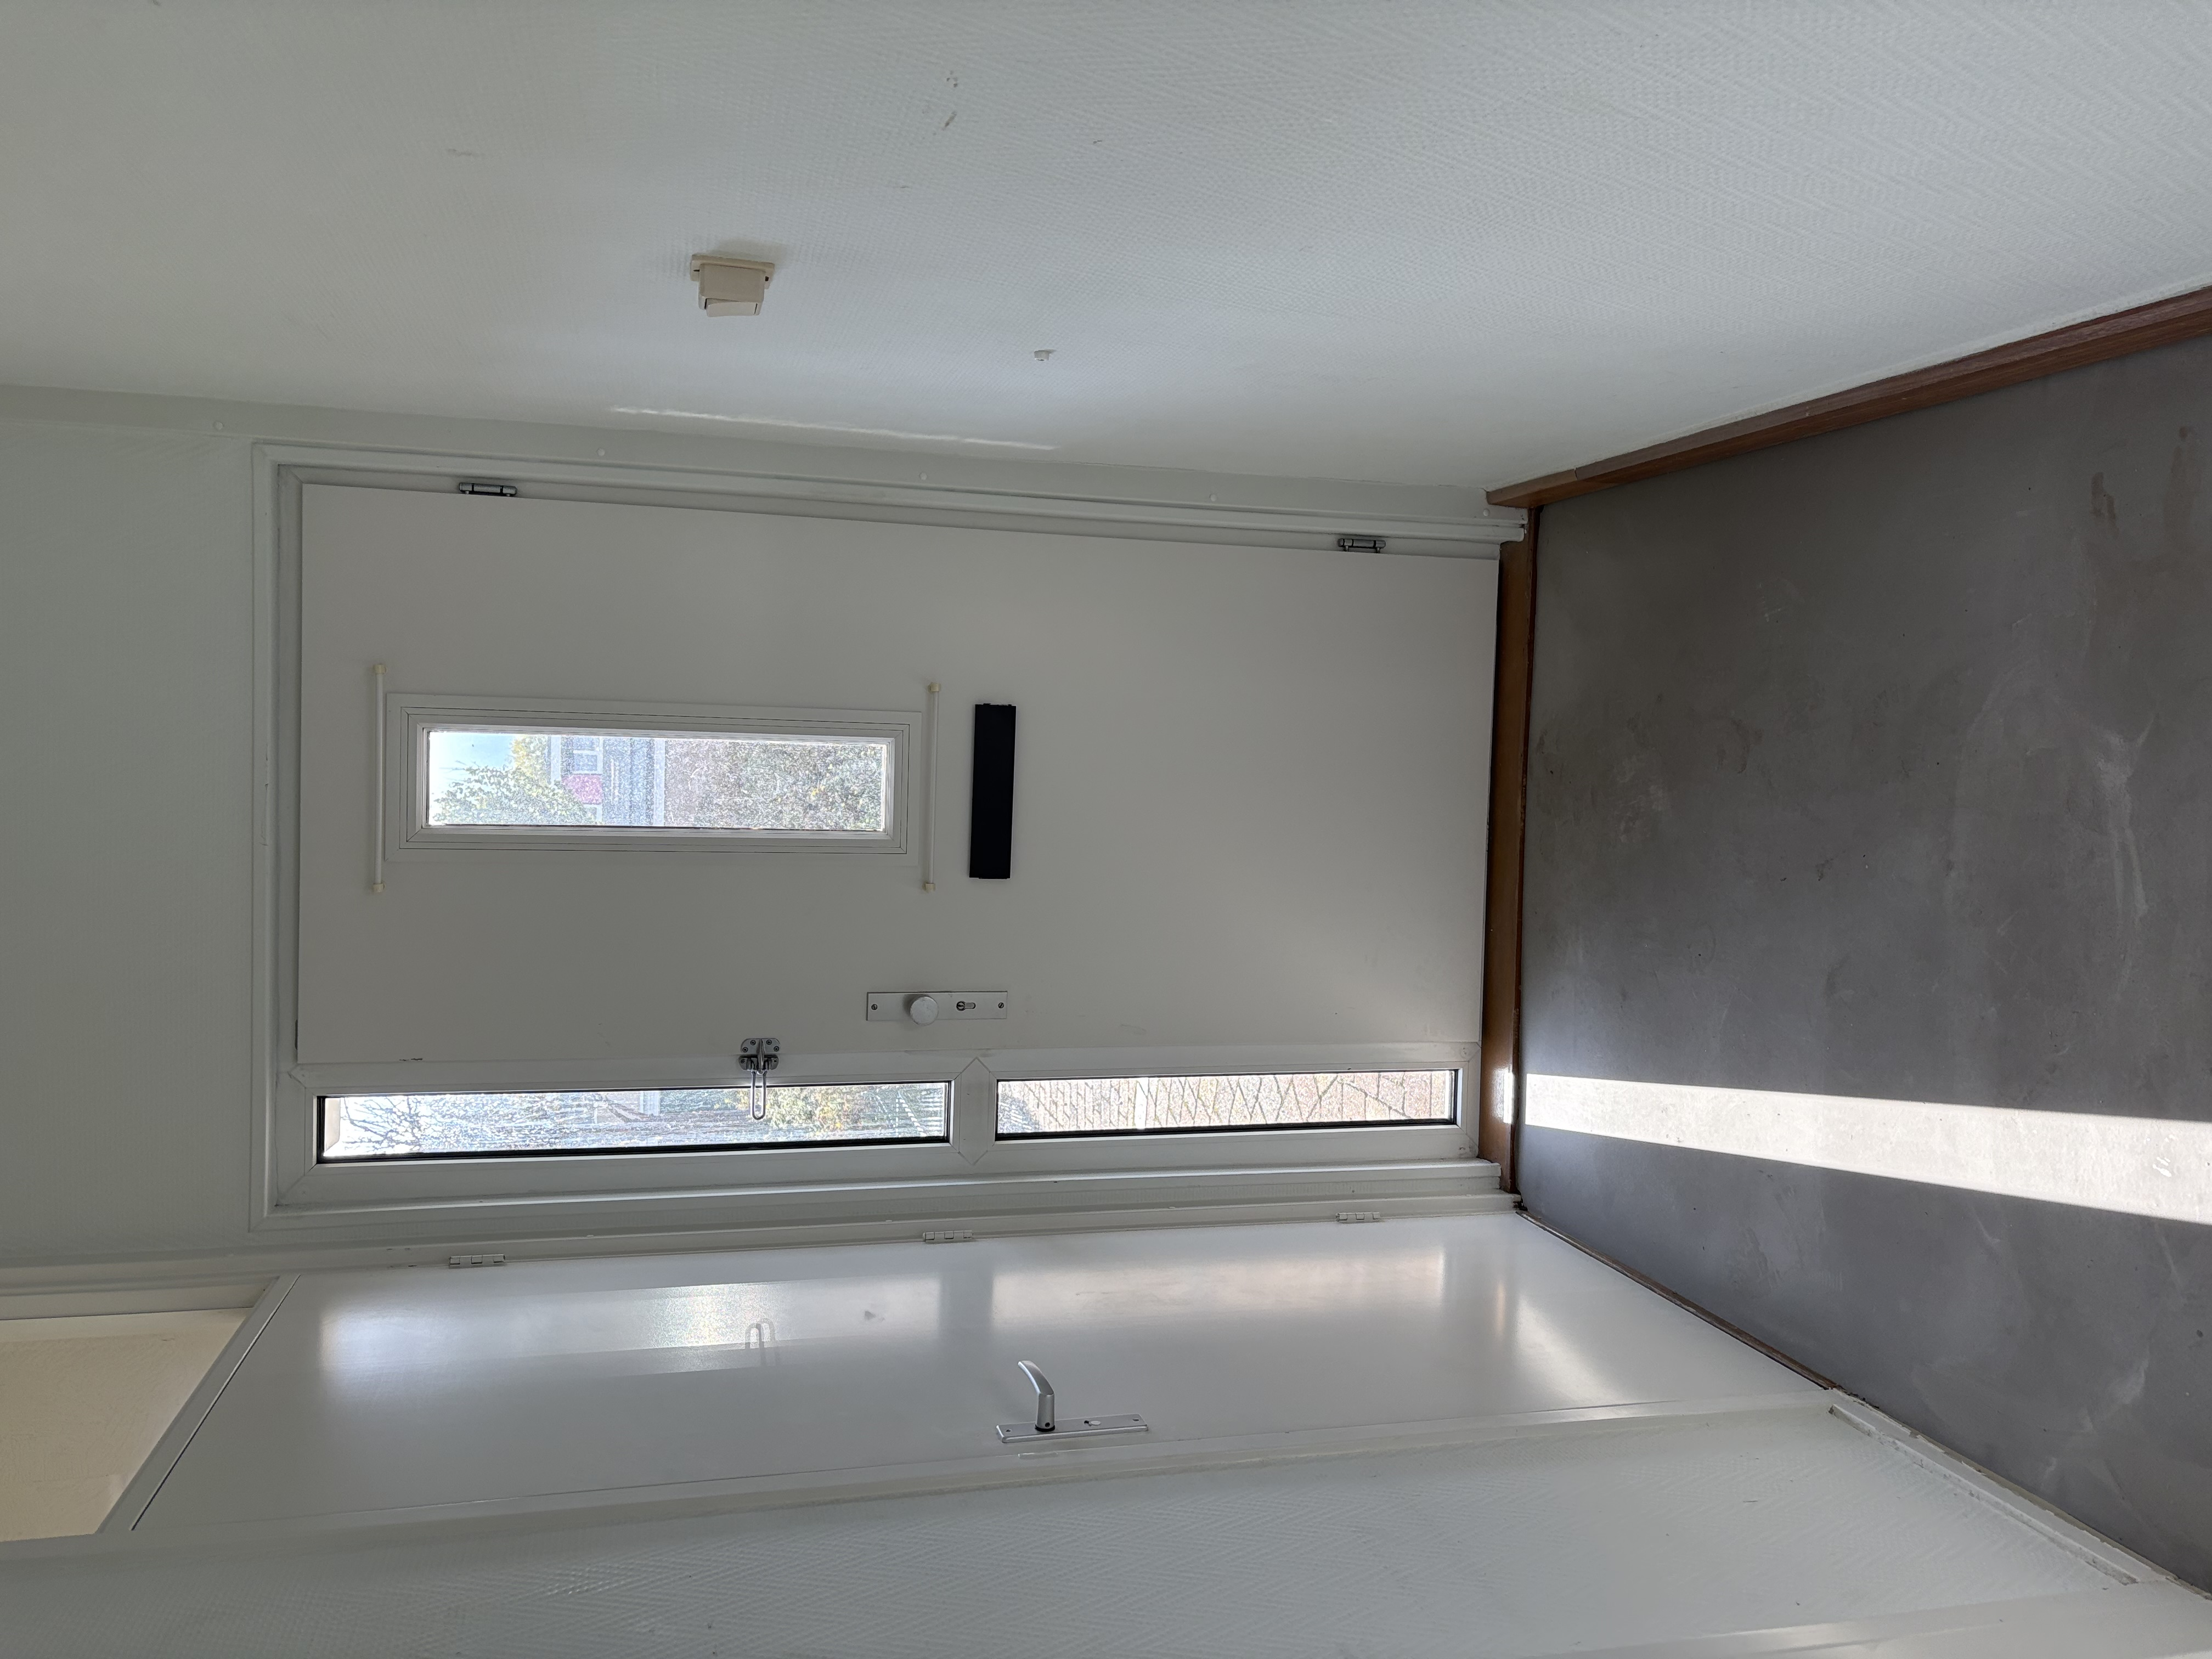
\includegraphics[angle=270,width=\linewidth]{sections/1-thesis-design/geenschade3.jpg}

        \small (c) Empty interior
    \end{minipage}

    \vspace{0.4cm}

    % Row 2
    \begin{minipage}{0.32\textwidth}
        \centering
        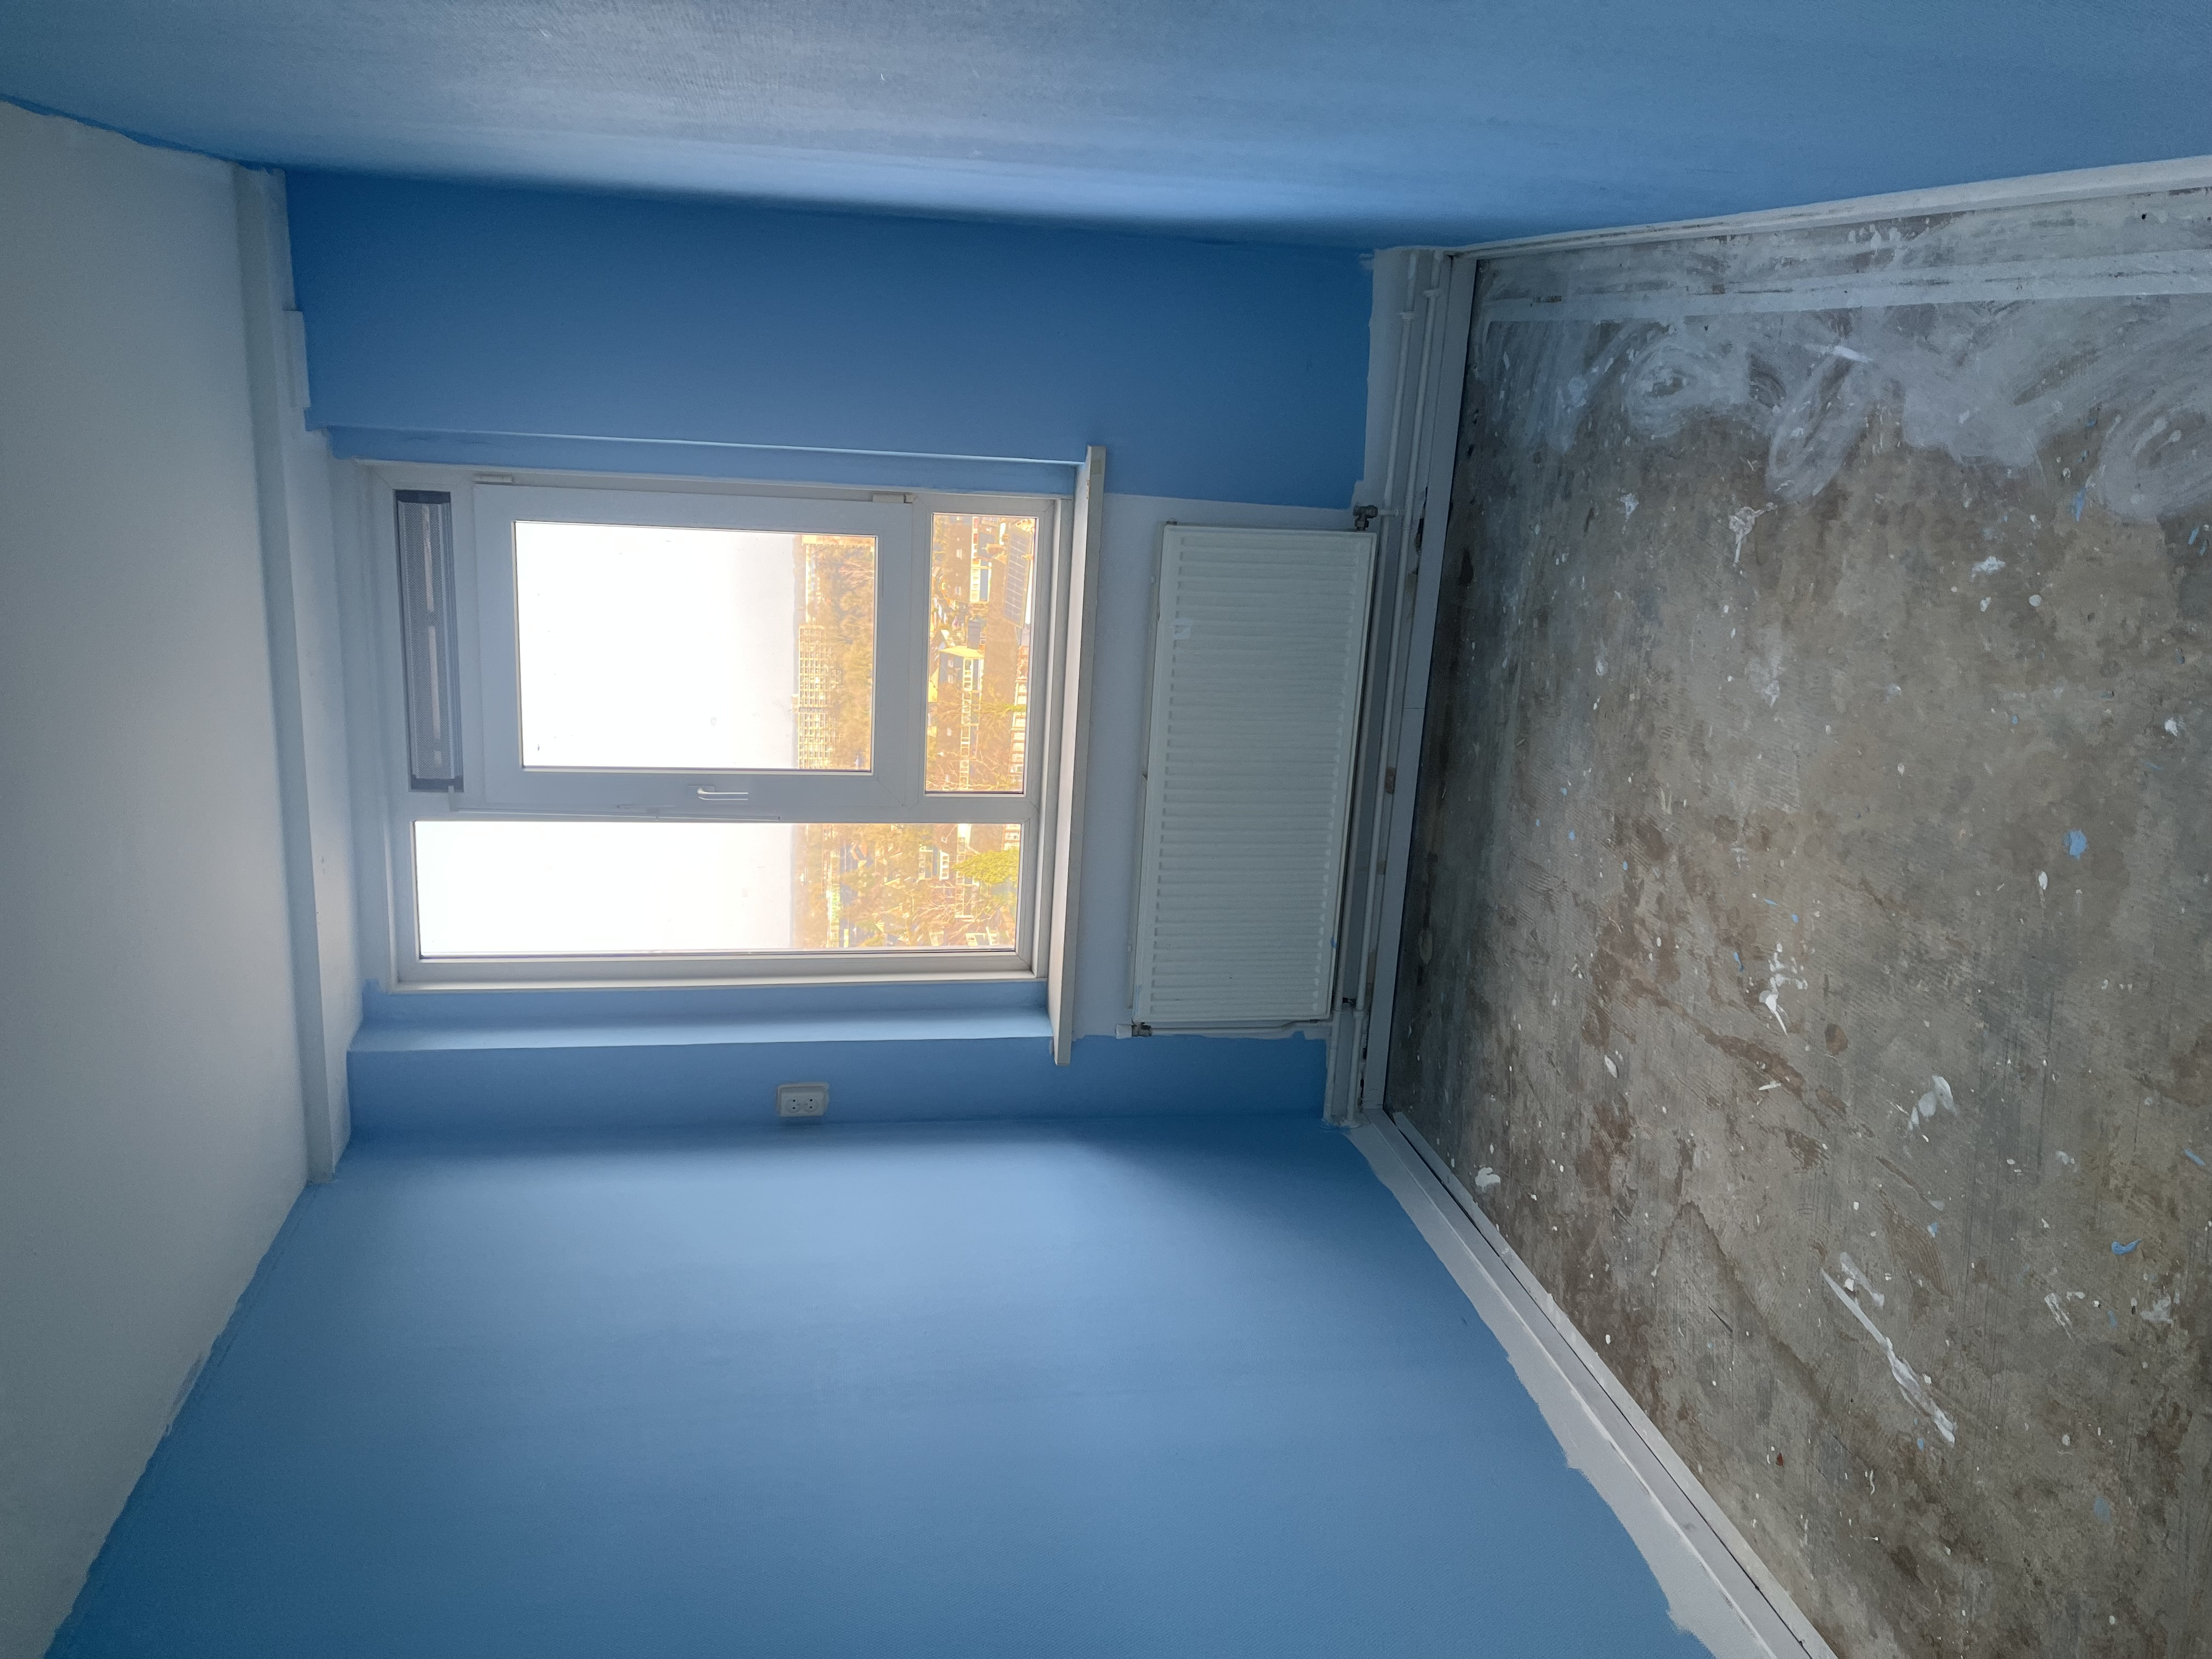
\includegraphics[angle=270,width=\linewidth]{sections/1-thesis-design/geen_schade.jpg}

        \small (d) Interior without damage
    \end{minipage}\hfill
    \begin{minipage}{0.32\textwidth}
        \centering
        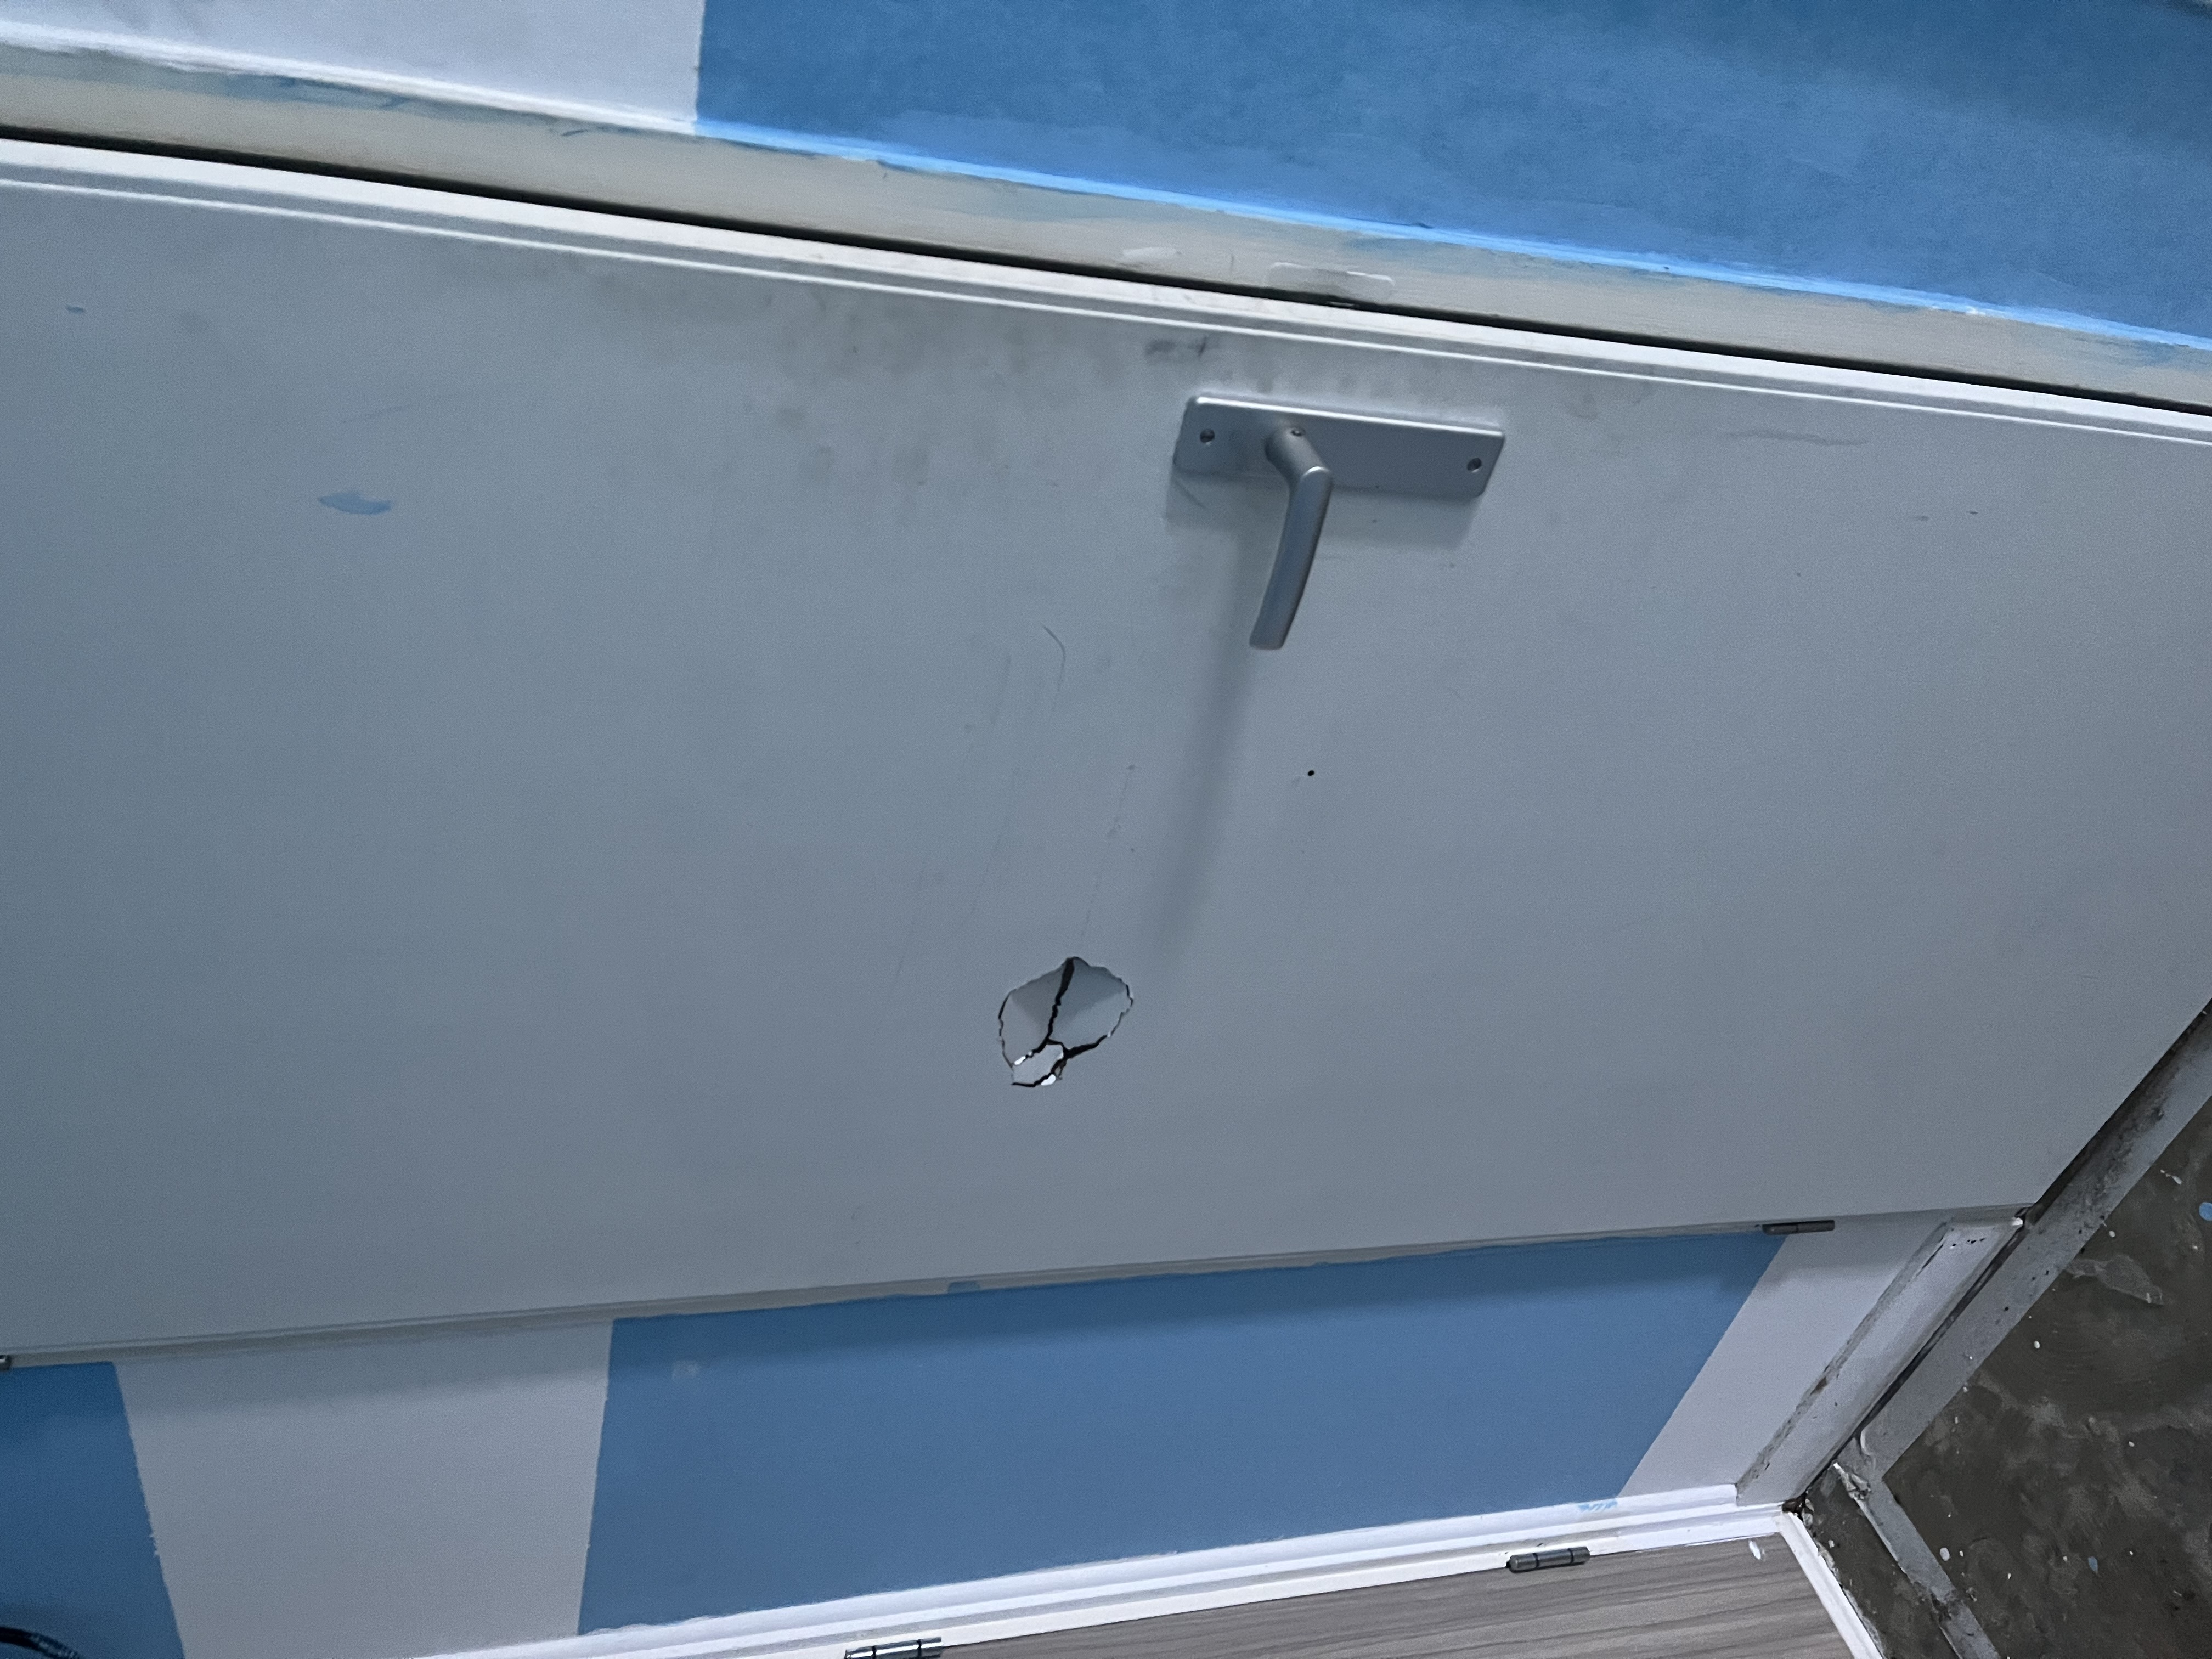
\includegraphics[angle=270,width=\linewidth]{sections/1-thesis-design/gat_in_deur.jpg}

        \small (e) Hole in door
    \end{minipage}\hfill
    \begin{minipage}{0.32\textwidth}
        \centering
        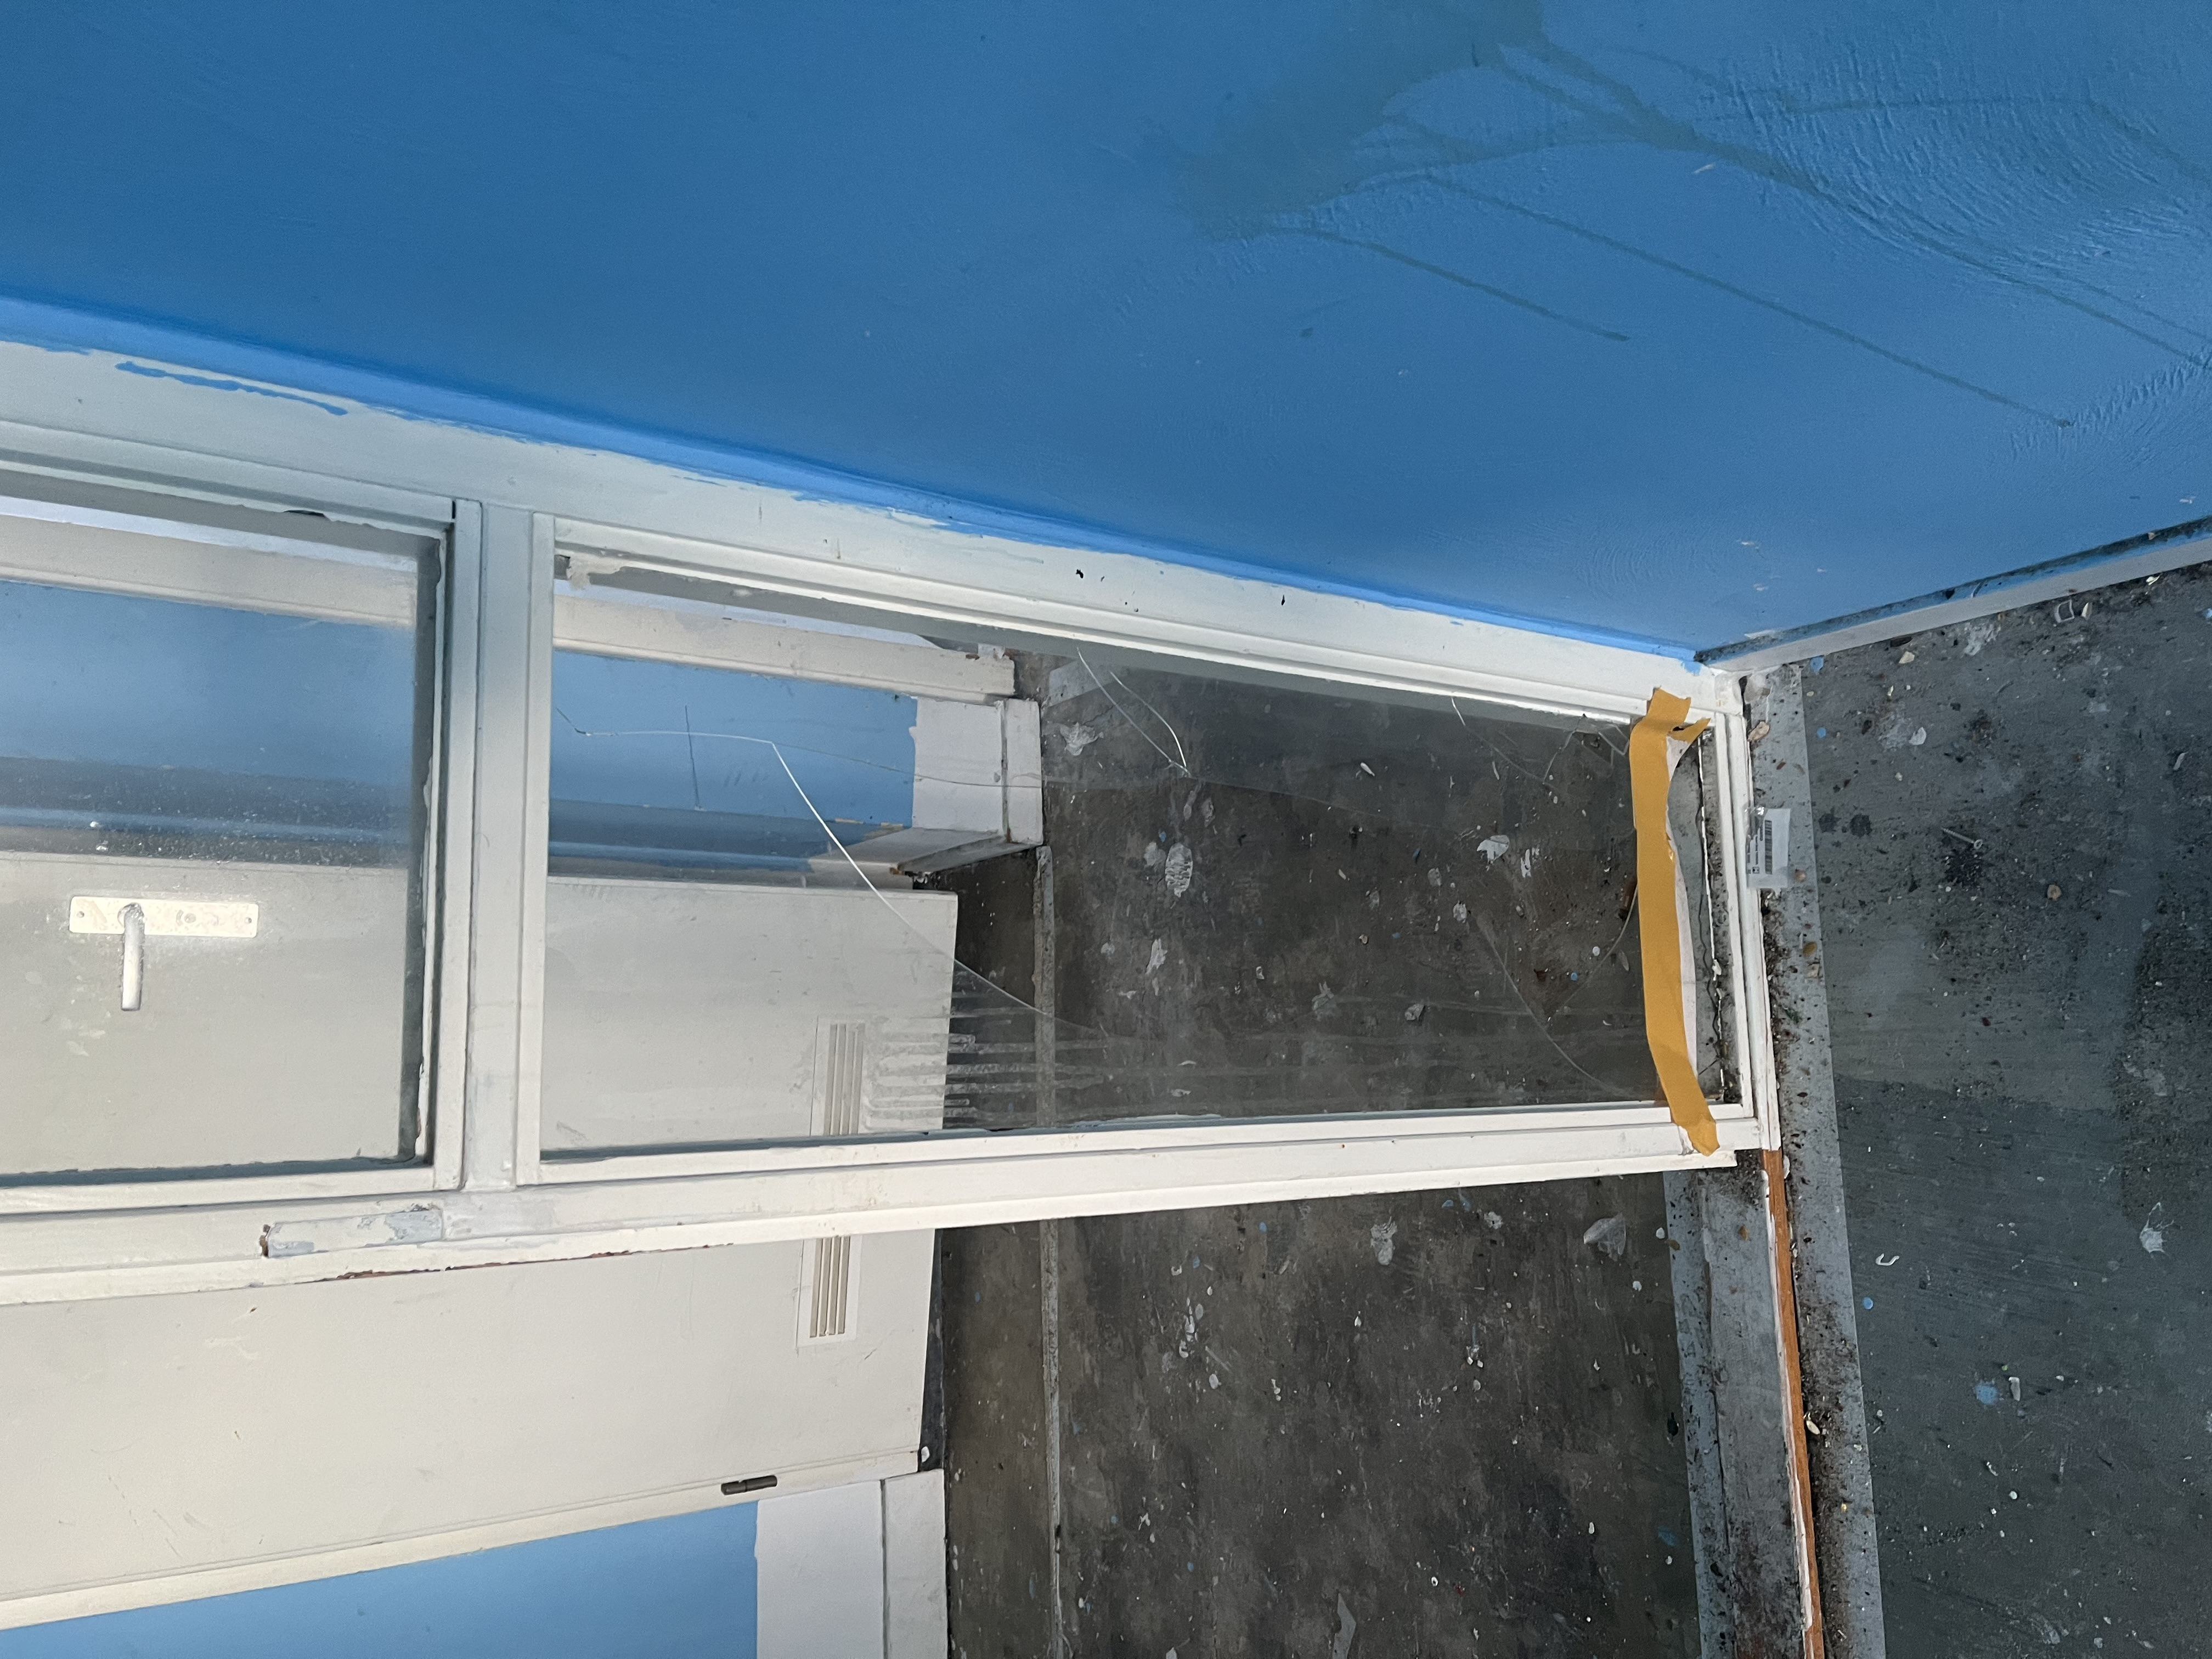
\includegraphics[angle=270,width=\linewidth]{sections/1-thesis-design/glas_en_muurschade.jpg}

        \small (f) Glass and wall damage
    \end{minipage}

    \vspace{0.4cm}

    % Row 3
    \begin{minipage}{0.32\textwidth}
        \centering
        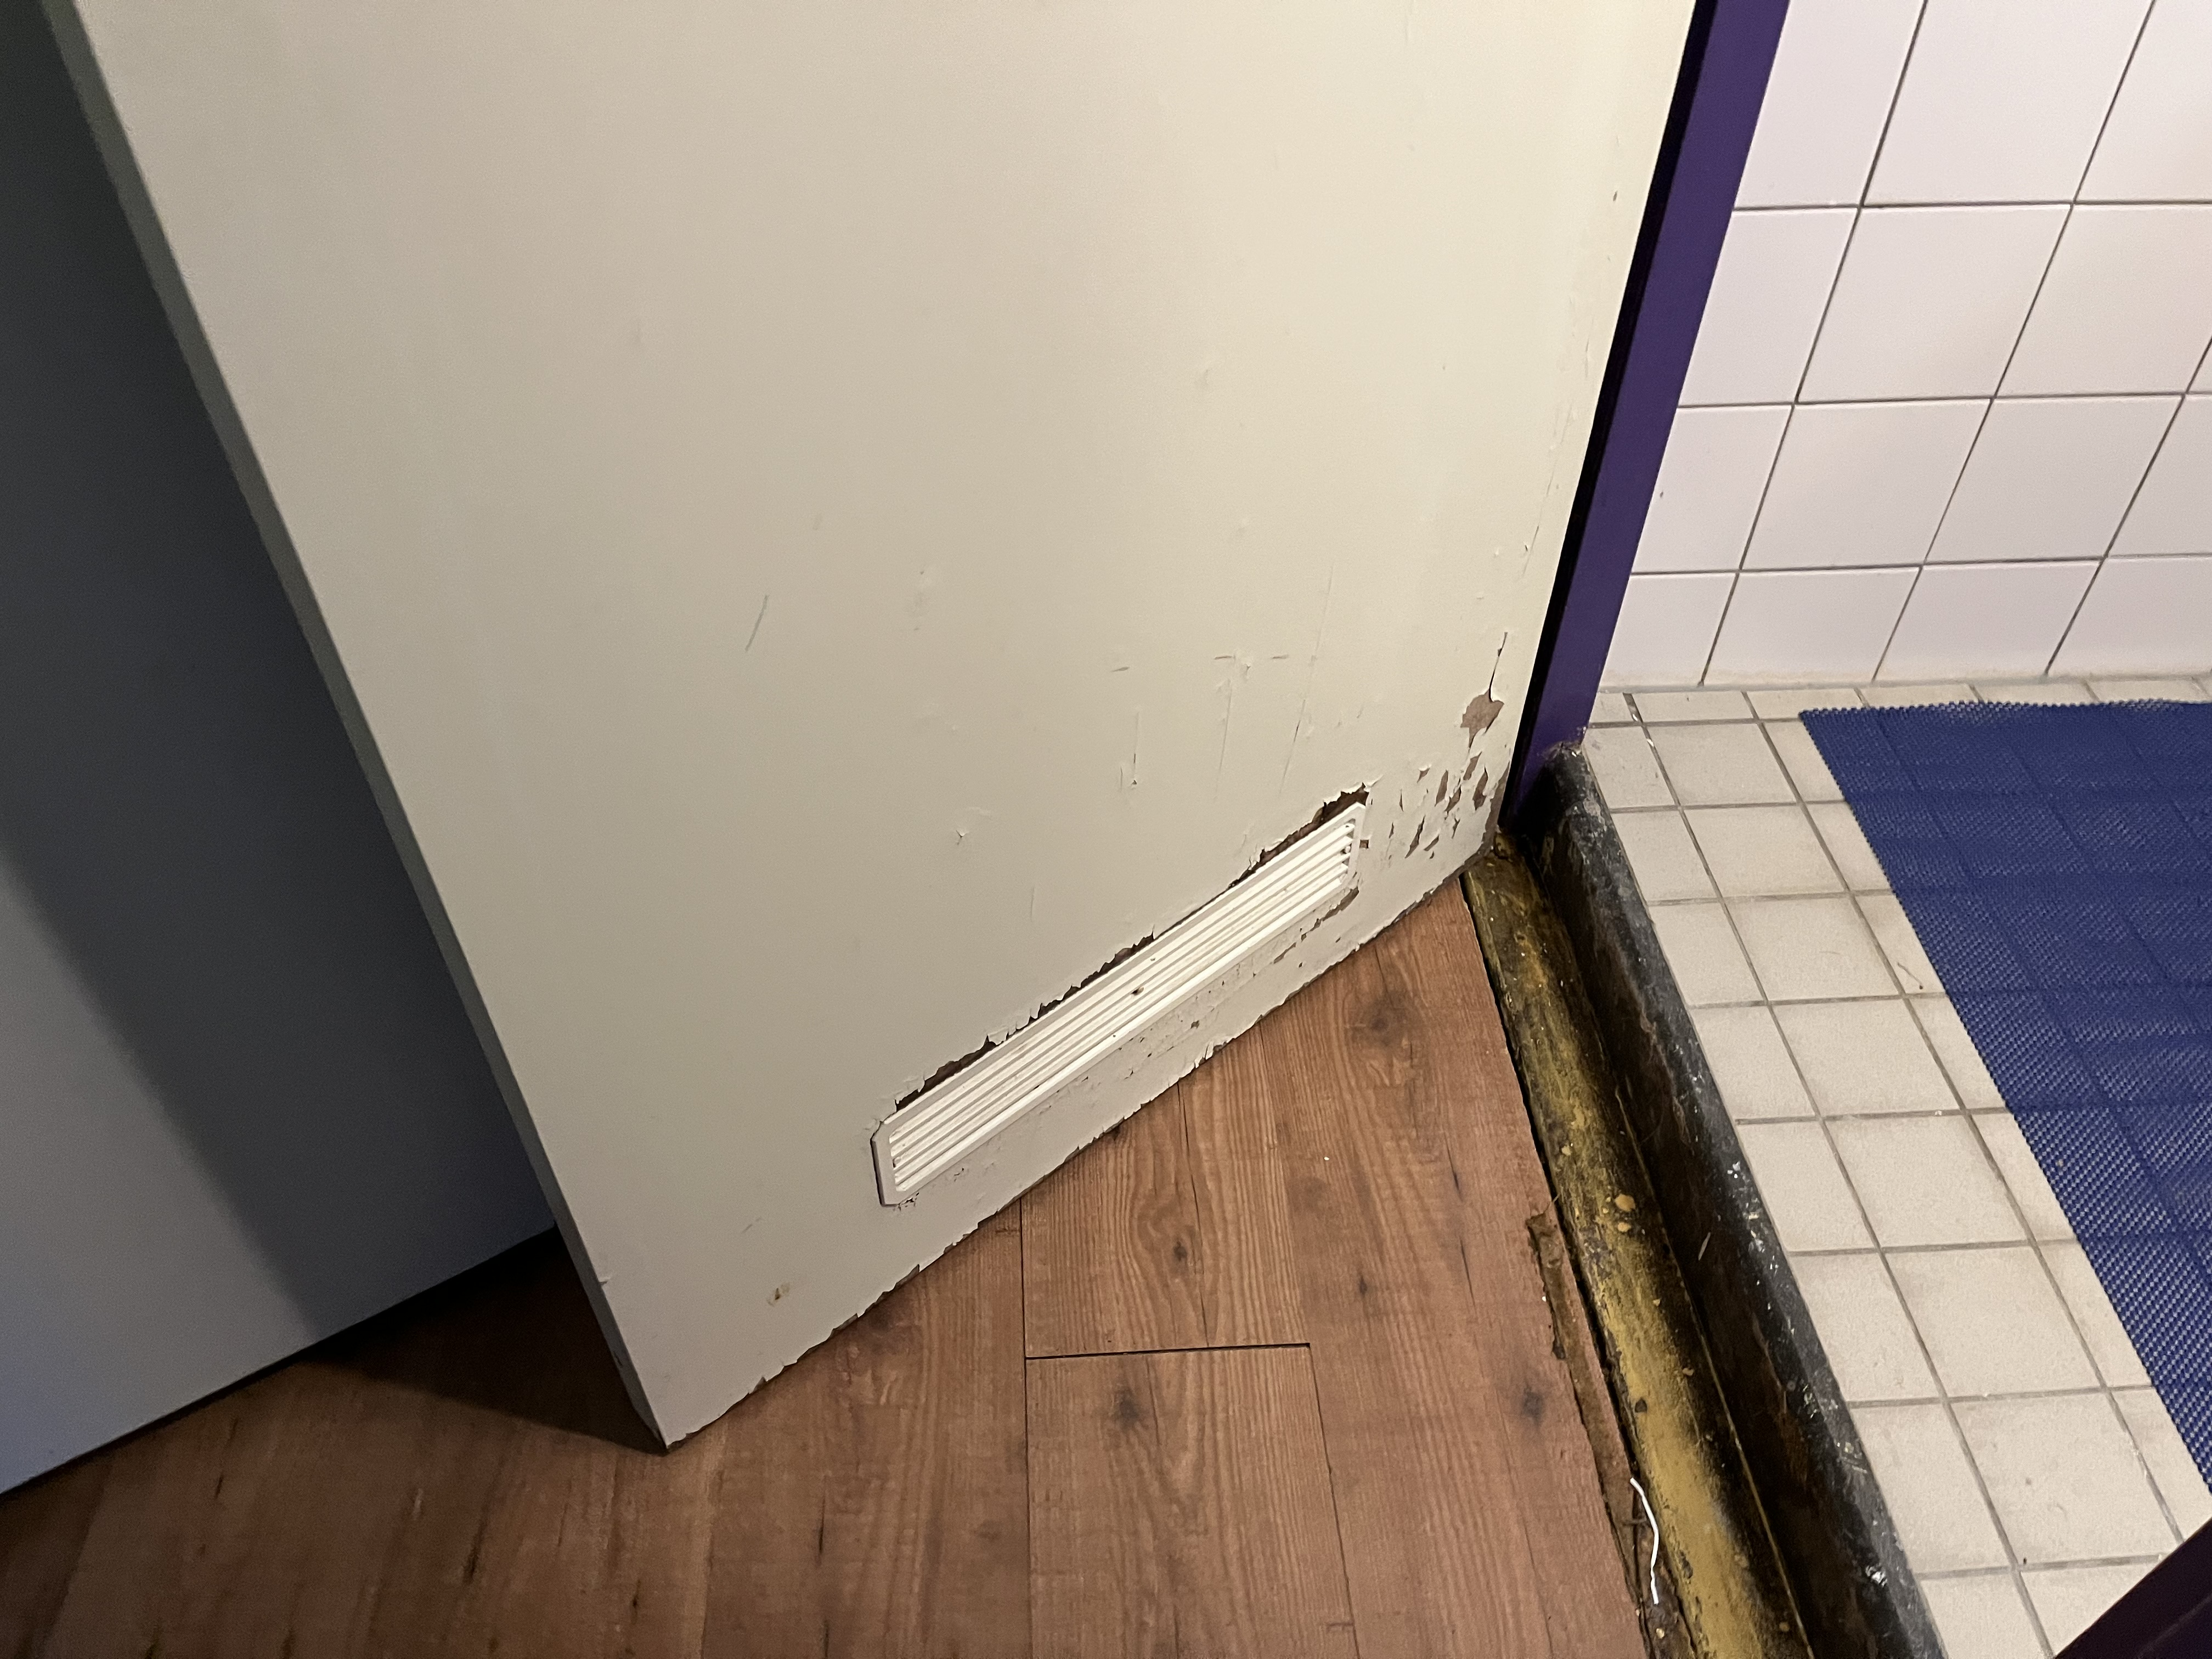
\includegraphics[angle=270,width=\linewidth]{sections/1-thesis-design/verf_schade.jpg}

        \small (g) Paint damage
    \end{minipage}\hfill
    \begin{minipage}{0.32\textwidth}
        \centering
        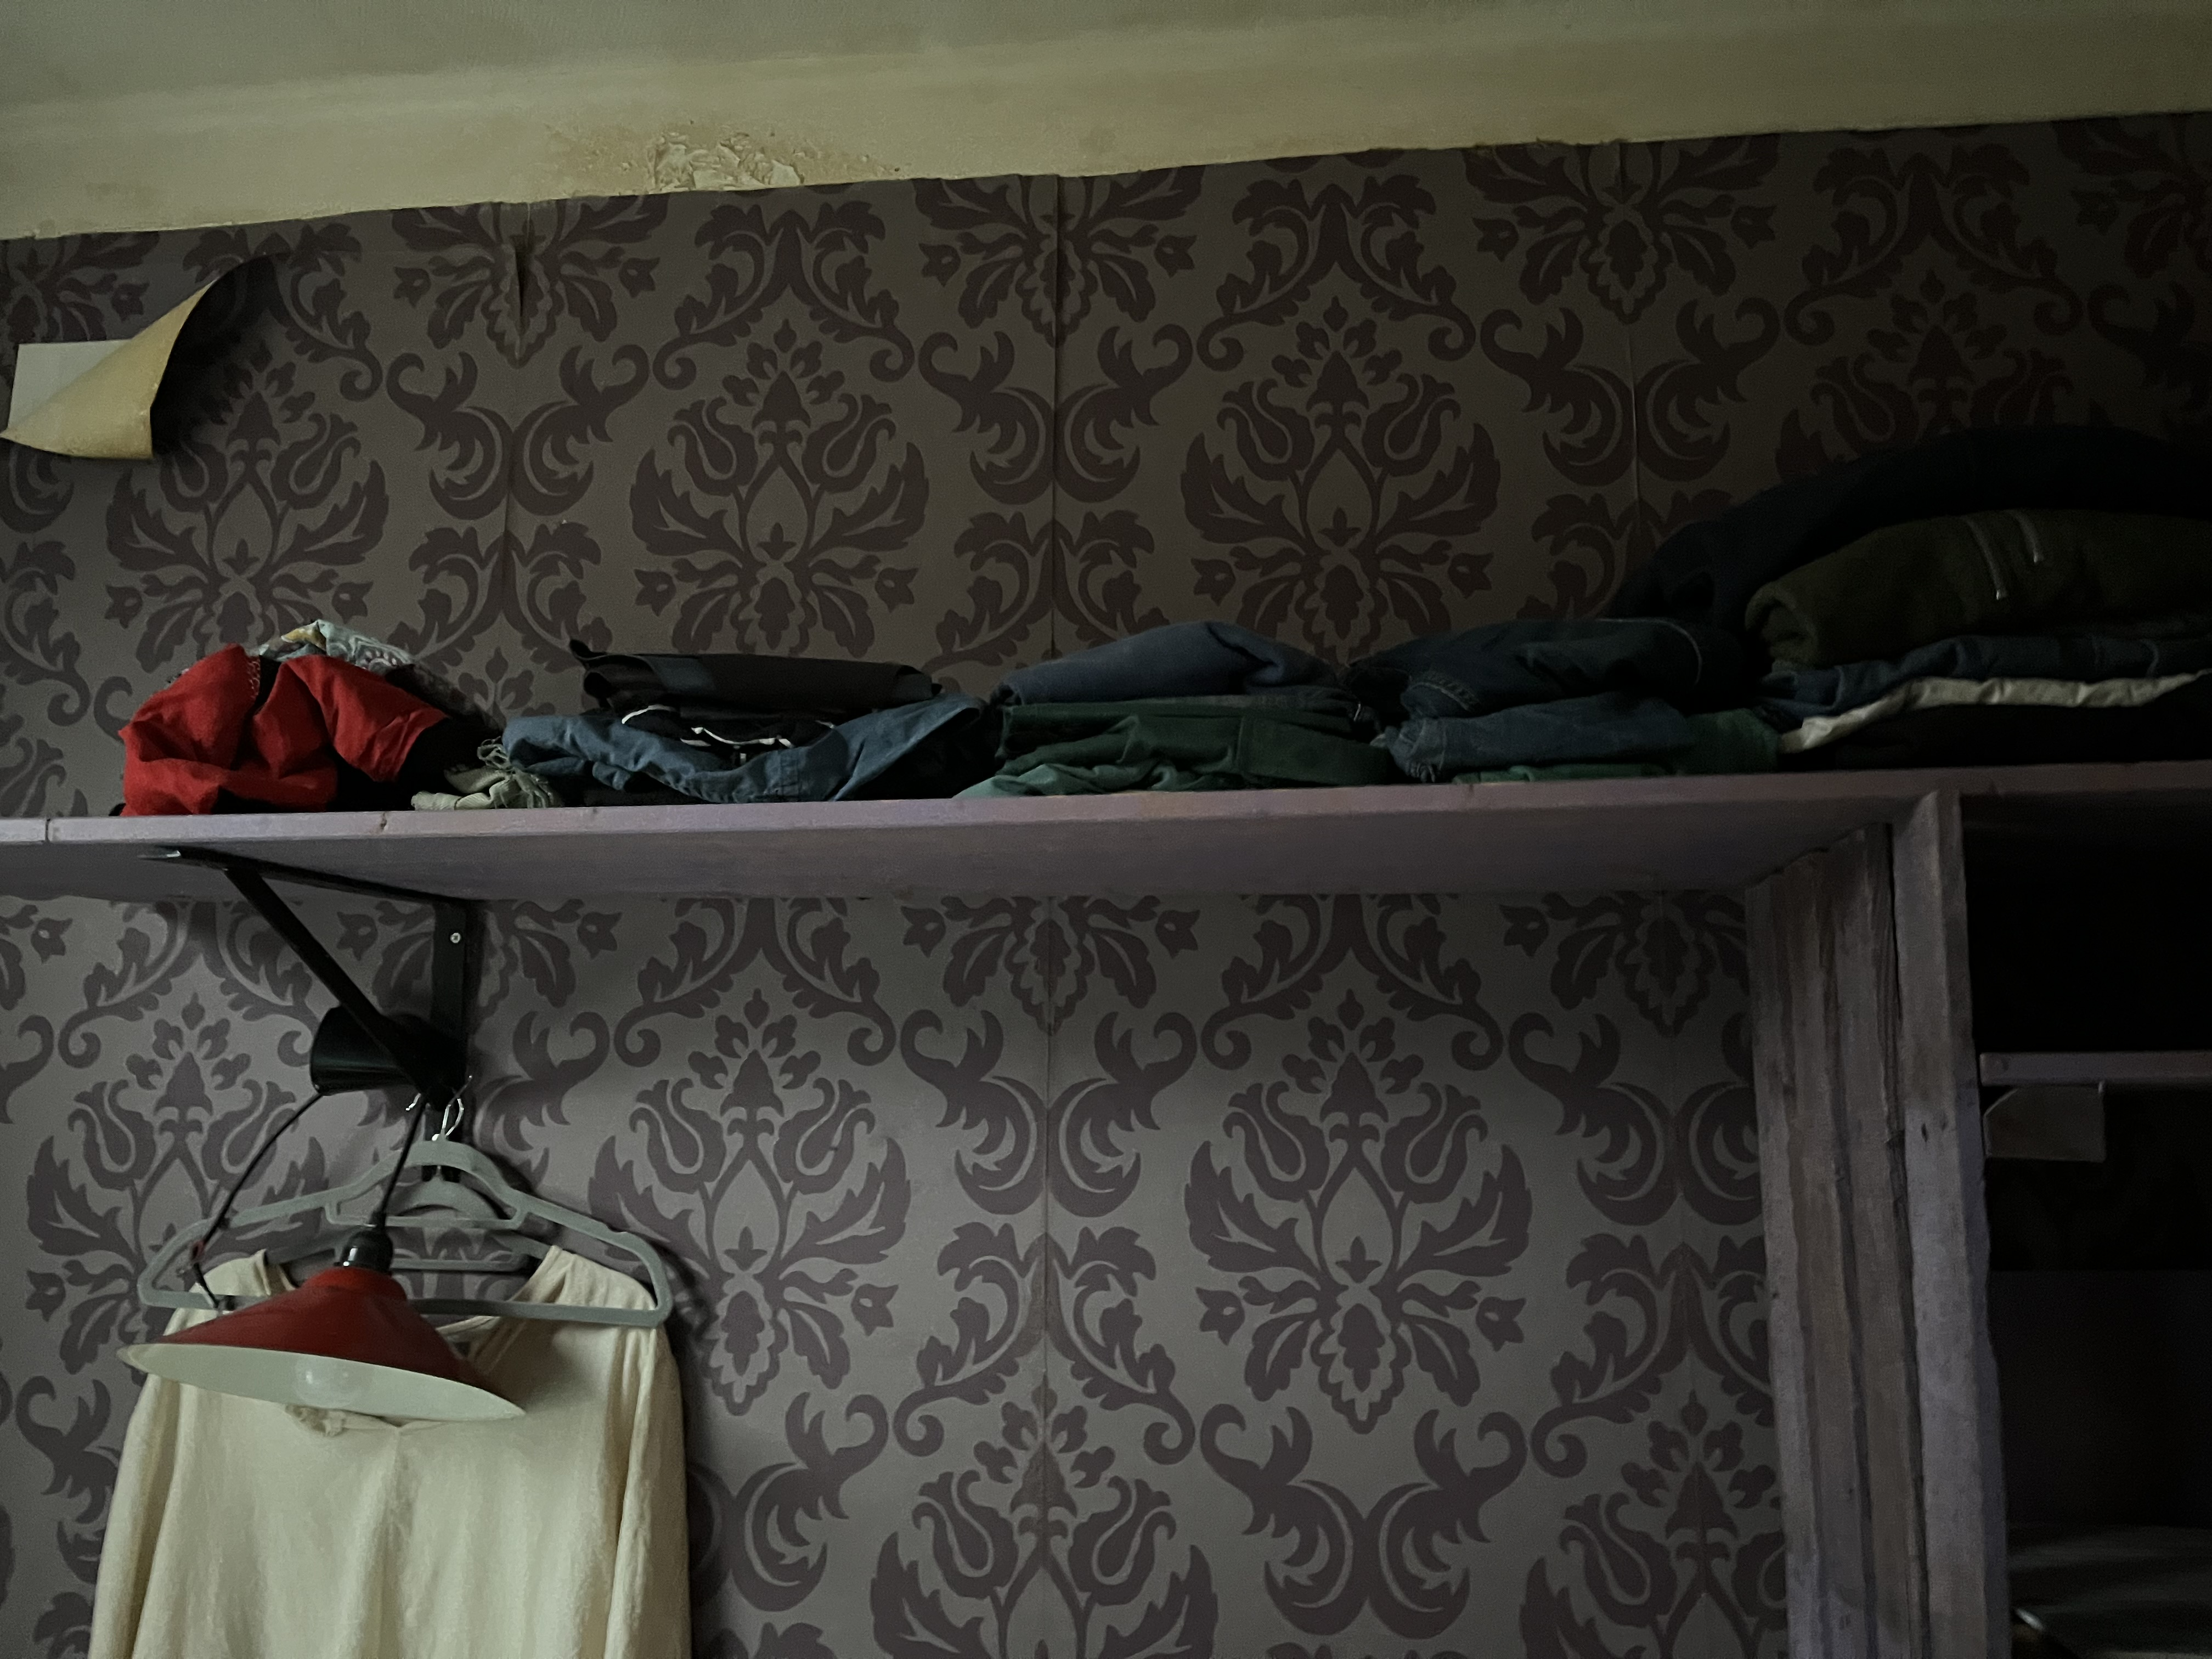
\includegraphics[angle=270,width=\linewidth]{sections/1-thesis-design/verf_en_behang_schade.jpg}

        \small (h) Paint and wallpaper damage
    \end{minipage}\hfill
    \begin{minipage}{0.32\textwidth}
        \centering
        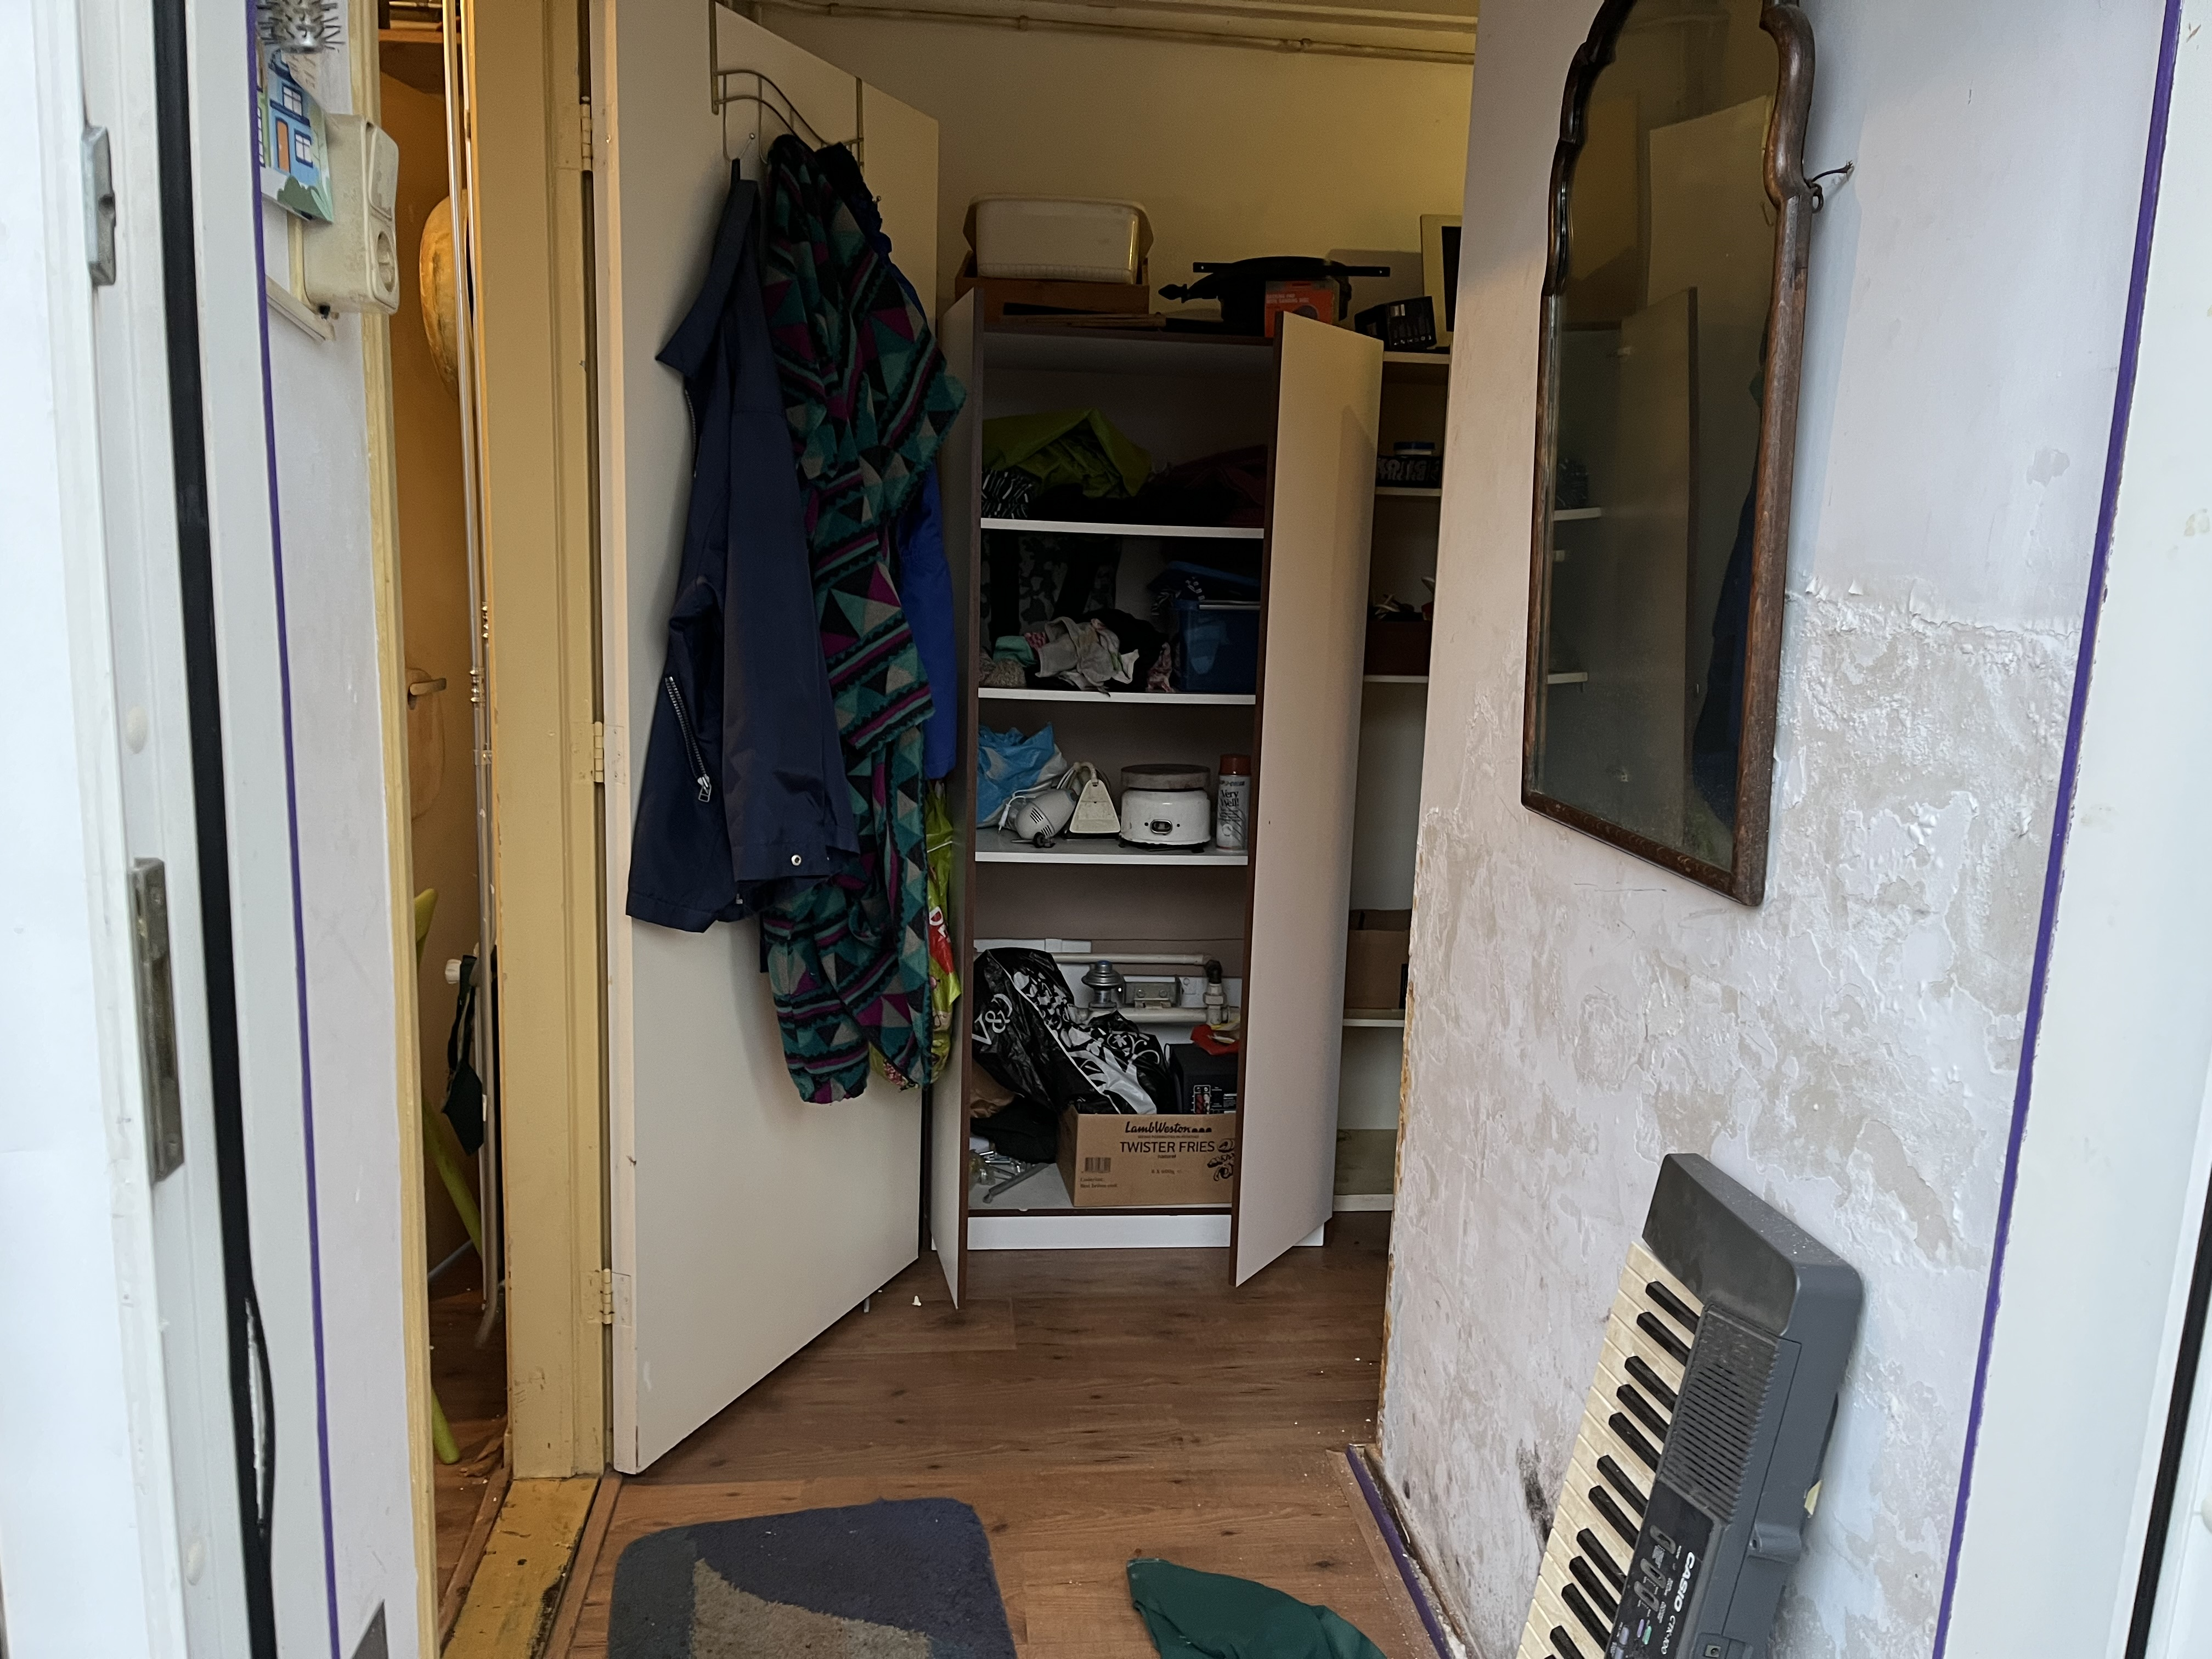
\includegraphics[angle=270,width=\linewidth]{sections/1-thesis-design/overlijden_schade.jpg}

        \small (i) Interior deterioration
    \end{minipage}

    \caption{Example inspection images from the DGW housing dataset.}
    \label{fig:dgw_examples}
\end{figure}
